\documentclass[12pt]{exam}
\usepackage[utf8]{inputenc}
\usepackage{cancel}
\usepackage{amsmath,amstext,amsthm,amssymb,amsxtra, graphicx}
\usepackage[top=1.5in, bottom=1.5in, left=1.25in, right=1.25in]	{geometry}
%\usepackage[normalem]{ulem}
\usepackage{pdfpages}
\usepackage{txfonts} % pxfonts txfonts 
\usepackage[T1]{fontenc}
\usepackage{lmodern}
\renewcommand*\familydefault{\sfdefault}
 \usepackage{euler}   % better than the option below
\usepackage{pdfsync}
\usepackage{multicol}
\newcommand{\ci}[1]{_{ {}_{\scriptstyle #1}}}
\graphicspath{ {images/} }


\newcommand{\norm}[1]{\ensuremath{\left\|#1\right\|}}
\newcommand{\abs}[1]{\ensuremath{\left\vert#1\right\vert}}
\newcommand{\ip}[2]{\ensuremath{\left\langle#1,#2\right\rangle}}
\newcommand{\p}{\ensuremath{\partial}}
\newcommand{\pr}{\mathcal{P}}

\newcommand{\pbar}{\ensuremath{\bar{\partial}}}
\newcommand{\db}{\overline\partial}
\newcommand{\D}{\mathbb{D}}
\newcommand{\B}{\mathbb{B}}
\newcommand{\Sp}{\mathbb{S}}
\newcommand{\T}{\mathbb{T}}
\newcommand{\R}{\mathbb{R}}
\newcommand{\Z}{\mathbb{Z}}
\newcommand{\C}{\mathbb{C}}
\newcommand{\N}{\mathbb{N}}
\newcommand{\Q}{\mathbb{Q}}
\newcommand{\mQ}{\mathcal{Q}}
\newcommand{\mS}{\mathcal{S}}
\newcommand{\scrH}{\mathcal{H}}
\newcommand{\scrL}{\mathcal{L}}
\newcommand{\td}{\widetilde\Delta}
\newcommand{\pw}{\text{PW}}
\newcommand{\esup}{\text{ess.sup}}
\newcommand{\Tn}{\mathcal{T}_n}
\newcommand{\Bn}{\mathbb{B}_n}
\newcommand{\rt}{\mathcal{O}}
\newcommand{\avg}[1]{\langle #1 \rangle}
\newcommand{\one}{\mathbbm{1}}
\newcommand{\eps}{\varepsilon}
\newcommand{\grad}{\nabla}

\newcommand{\La}{\langle }
\newcommand{\Ra}{\rangle }
\newcommand{\rk}{\operatorname{rk}}
\newcommand{\card}{\operatorname{card}}
\newcommand{\ran}{\operatorname{Ran}}
\newcommand{\osc}{\operatorname{OSC}}
\newcommand{\im}{\operatorname{Im}}
\newcommand{\re}{\operatorname{Re}}
\newcommand{\tr}{\operatorname{tr}}
\newcommand{\vf}{\varphi}
\newcommand{\f}[2]{\ensuremath{\frac{#1}{#2}}}

\newcommand{\kzp}{k_z^{(p,\alpha)}}
\newcommand{\klp}{k_{\lambda_i}^{(p,\alpha)}}
\newcommand{\TTp}{\mathcal{T}_p}
\newcommand{\m}[1]{\mathcal{#1}}
\newcommand{\md}{\mathcal{D}}
\newcommand{\qan}{\abs{Q}^{\alpha/n}}
\newcommand{\sbump}[2]{[[ #1,#2 ]]}
\newcommand{\mbump}[2]{\lceil #1,#2 \rceil}
\newcommand{\cbump}[2]{\lfloor #1,#2 \rfloor}

\newcommand{\hn}{{3}}
\newcommand{\dd}{{10-06}}
\newcommand{\class}{Aero 417}
\newcommand{\term}{Fall 2024}
\newcommand{\examnum}{Homework \hn: Due \dd}
\newcommand{\examdate}{}
\newcommand{\timelimit}{75 Minutes}
\newcommand{\vc}[3]{\langle #1,#2,#3\rangle}
\newcommand*{\vv}[1]{\vec{\mkern0mu#1}}
\newcommand{\bv}[1]{\boldsymbol{#1}}
\newcommand{\hide}[1]{}
\newcommand{\uvec}[1]{\boldsymbol{\hat{\textbf{#1}}}}
\newcommand{\vex}[1]{\boldsymbol{{\textbf{#1}}}}
\newcommand{\px}{\frac{\partial}{\partial x}}
\newcommand{\py}{\frac{\partial}{\partial y}}
\newcommand{\pt}{\frac{\partial}{\partial t}}
\newcommand{\pxx}{\frac{\partial^2}{\partial x^2}}
\newcommand{\pyy}{\frac{\partial^2}{\partial y^2}}
\newcommand{\ptt}{\frac{\partial^2}{\partial t^2}}


\pagestyle{head}
\firstpageheader{}{}{}
\runningheader{\class}{ Page \thepage\ of \numpages}{\examnum}
\runningheadrule

\makeatletter
\renewcommand*\env@matrix[1][*\c@MaxMatrixCols c]{%
  \hskip -\arraycolsep
  \let\@ifnextchar\new@ifnextchar
  \array{#1}}
\makeatother

\printanswers
\begin{document}

\noindent
\begin{tabular*}{\textwidth}{l @{\extracolsep{\fill}} r @{\extracolsep{6pt}} l}
\textbf{\class} & \textbf{Name:} & \makebox[2in]{\bf{Benjamin Tollison}}\\
\end{tabular*}\\
\rule[2ex]{\textwidth}{2pt}
%
\begin{questions}
\begin{question}
Why centrifugal compressors are not used in long-range aircraft as a component of the main
engines?
\end{question}
\begin{solutionorbox}[\stretch{1}]
Starting with the breguet's range equation:
\[S = \frac{L}{D} \eta_0 \frac{\text{LHV}}{g} \ln \left(\frac{m_0}{m_f}\right)\]
We will assume that the aircraft will have the same take-off weight and same dry weight and the 
only thing that we are changing is going to be the compressor geometry. Therefore the compressor
will only effect the overall efficency \(\eta_0\), and \(\eta_0 \propto \eta_c\).
\[\rightarrow S \propto \eta_c\]
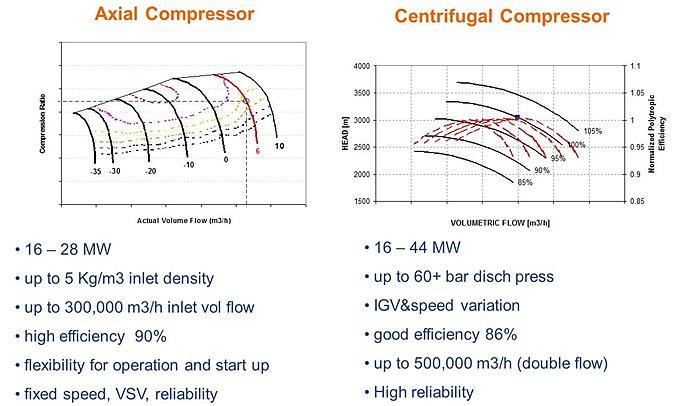
\includegraphics[width=\linewidth]{Axial-vs-Centrifugal-Compressor-Comparison.jpg}
because every little bit of efficency matters over the lifetime of the engine flight time
to save millons on fuel. That it makes sense that modern commerical jet would prefer for 
an axial compressor over a centrifugal one.
\end{solutionorbox}

\newpage 
\begin{question}
Explain, using mathematical expressions the source of pressure increases in a centrifugal
compressor and make a reflection and describe what is the source/term that indicates the
pressure increase in high performance centrifugal compressors
\end{question}
\begin{solutionorbox}[\stretch{1}]
Assume: adiabatic, incompressible, quasi-1D flow, steady state

\begin{center}
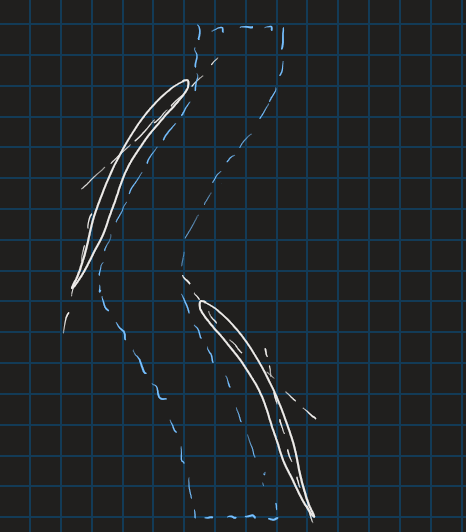
\includegraphics[width=200pt]{Compressor control volume.png}
\end{center}
Starting with the conservation of mass:
\[\int_{\tau} \partial_t \rho \, d\tau + \int_{\sigma} \rho (\vec{v} \cdot \vec{n}) \, d\sigma = 0\]
\[-\rho_1 v_1 \sigma_1 + \rho_2 v_2 \sigma_2 = 0\]
\[\therefore \dot{m_1} = \dot{m_2} \quad \text{or} \quad v_1 \sigma_1 = v_2 \sigma_2\]
After getting that relation we can use the momentum equation to produce the following
\[\int_{\tau} \partial_t (\rho \vec{v}) \, d\tau + \int_{\sigma} \rho \vec{v} (\vec{v} \cdot \vec{n}) \, d\sigma = \vec{F}_\nu + \vec{F}_s\]
\[
\begin{cases}
  \vec{F}_v = 0, \text{ neglected} \\
  \vec{F}_s = - \oint_{\sigma} P \cdot \vec{n} \, d\sigma = \Delta P \sigma
\end{cases}
\]
\[\Delta{P} = \frac{\dot{m}}{\sigma}\left(v_2-v_1\right)\]
The changes in pressure are going to be related based off of the difference in velocity
of the outlet versus the inlet with the current assumptions that I made.
\end{solutionorbox}


\newpage 
\begin{question}
Air enters the inducer blades of a centrifugal compressor at p01 = 1.02 bar, T01 = 335 K. The
hub and tip diameters of the impeller eye are 10 and 25 cm respectively. If the compressor
runs at 7200 rpm and delivers 5.0 kg/s of air, determine the air angle at the inducer blade
entry and the relative Mach number. 
\end{question}
\begin{solutionorbox}[\stretch{1}]
Starting by finding the annulus area

\[\frac{d}{dr} \left( \pi r^2 \right) = 2 \pi r\]
\[\sigma_1 = 2 \pi \int_{0.1}^{0.25} r \, dr \quad \left[ m^2 \right]\]
\[u_1 = 7200 \, \text{[rpm]} \left( \frac{2 \pi \, \text{[rads]}}{60 \, \text{[sec]}} \right)\]
Then solving the continuity equation
\[\cancelto{0}{\int_{\tau} \partial_t \rho \, d\tau} + \oint_{\sigma} \rho (\vec{v} \cdot \vec{n}) \, d\sigma = 0
\quad \text{(steady state)}\]
\[-\rho_1 v_1 \sigma_1 + \rho_2 v_2 \sigma_2 = 0 \quad \Bigg| \, v_1 = w_1, \quad \sigma_1 = \sigma_2\]
\[\dot{m}_1 = \dot{m}_2\]
Using the dimensionaless mass flow rate equation [Cizmas equation 3.39] to find the mach number via Newton Raphson.
My numerical scheme is the following
\[\zeta = -\frac{\dot{m}\sqrt{R T_0}}{P_0 \sigma} + \sqrt{\gamma} M \left( 1 + \frac{\gamma-1}{2} M^2 \right)^{-\frac{(\delta+1)}{2(\delta-1)}} = 0
\]
\[
\frac{d\zeta}{dM} = \sqrt{\gamma} \left( 1 + \frac{\gamma-1}{2} M^2 \right)^{-\frac{(\gamma+1)}{2(\gamma-1)}} 
\]\[ -\sqrt{\gamma} \mathcal{M} \left( \frac{(\gamma+1)}{2(\gamma-1)} \right) \left( 1 + \frac{\gamma-1}{2} M^2 \right)^{-\frac{(\gamma+1)}{2(\gamma-1)} - 1} 
\left( [\gamma - 1] M \right)
\]
\[M_{i+1} = M_i - \frac{\zeta}{\frac{d\zeta}{dM}}
\]
\[e_r = \left| \zeta(M_{i+1}) \right| > 1e-8
\]
Which produces a \(M = 3.5971\), and using \(w_1 = M\sqrt{\gamma R T_0}\) we can get the relative velocity of \(w_1 = 1319.7128 \left[\frac{m}{s}\right]\). Using trig we can find that 
\[\beta = \cos^-1\left(\frac{u_1}{w_1}\right)\]
therefore the final answers are the following
\begin{align*}
\begin{cases}
  M = 3.5971\\
  \beta_1 = 0.9627 \left[rads\right]\\
  \beta_1 = 55.15747^\circ
\end{cases}
\end{align*}

\end{solutionorbox}

\end{questions}
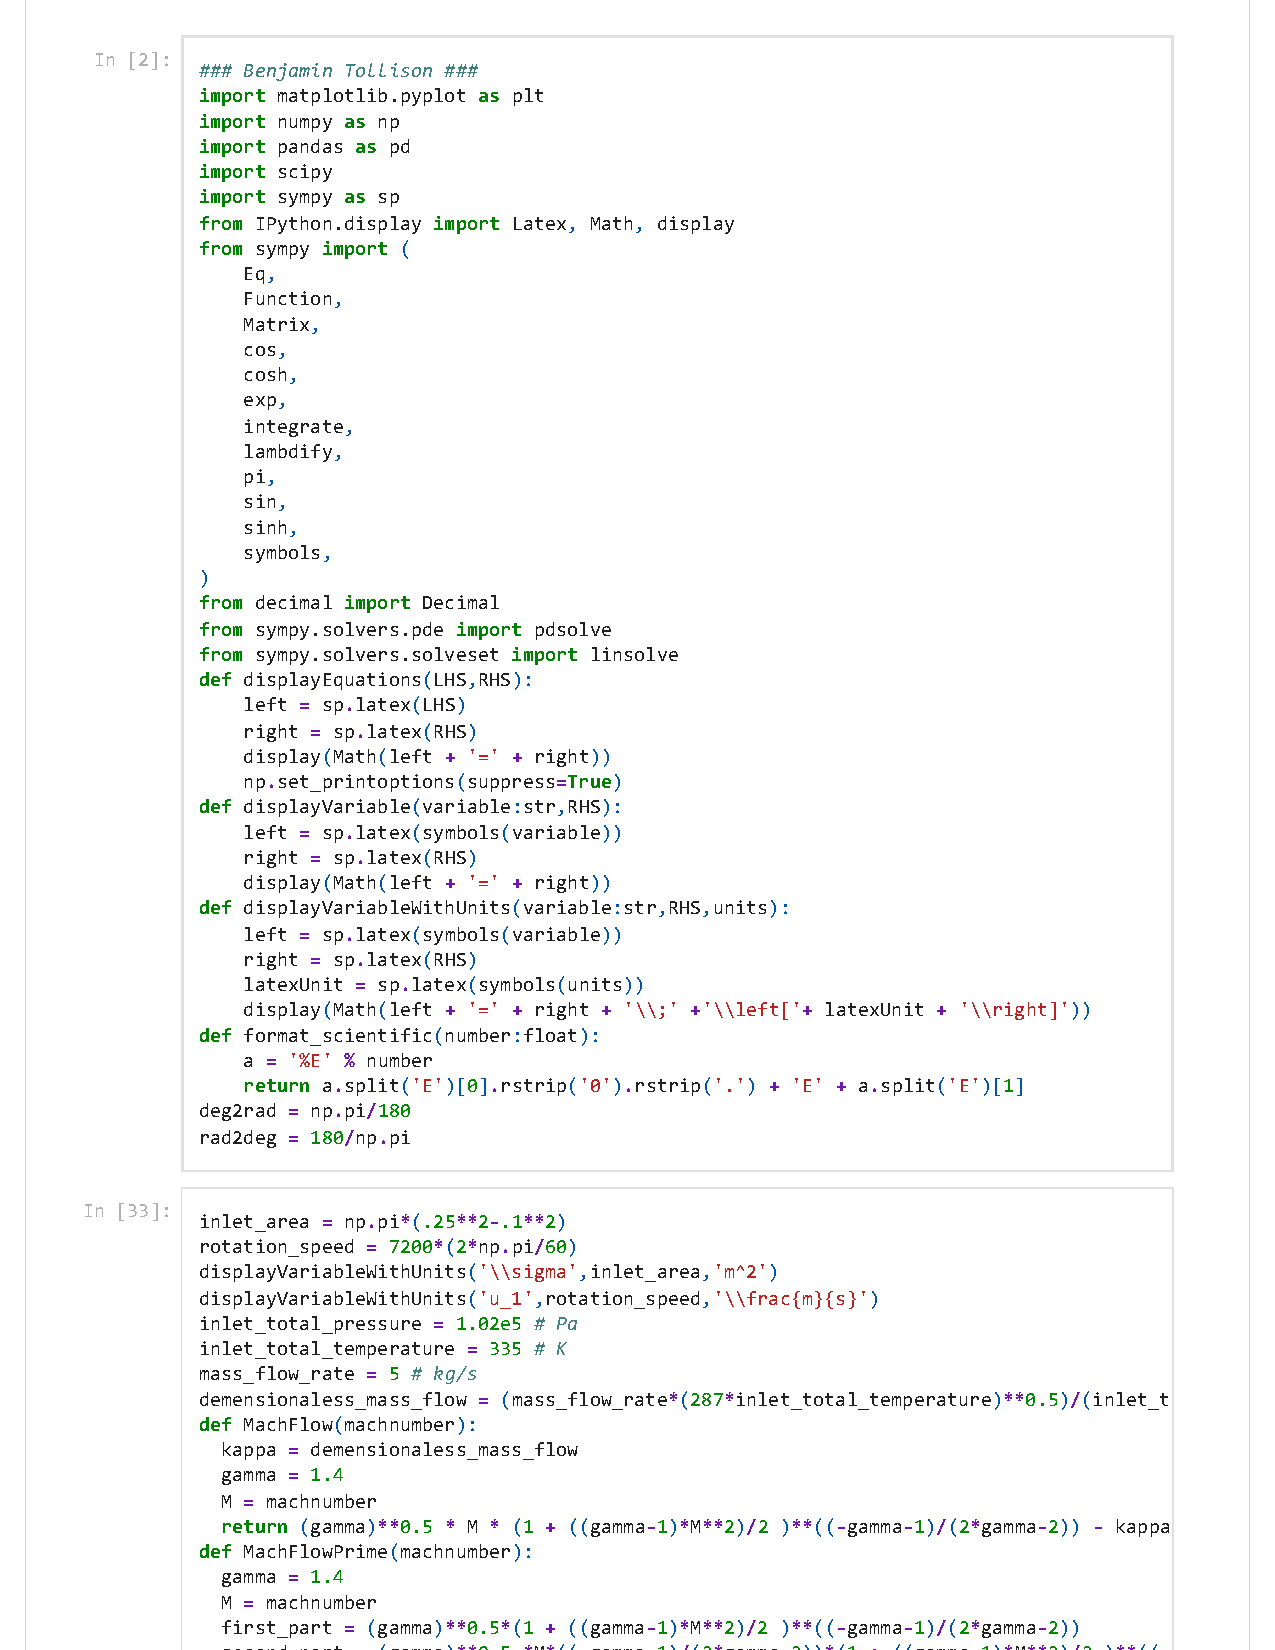
\includepdf[pages=-]{hw-3-code.pdf}
\end{document}
